% STC 720 research article: Stage 1 scaffold (30 Oct 2026).
% Structure and page budgets follow docs/STC720_assignment_rubric.pdf.
% Tables are generated by scripts/paper_assets.py from frozen results; do not edit report/tables/*.tex by hand.
% Build: latexmk -pdf main.tex   (from report/)
\documentclass[11pt,a4paper]{article}
\usepackage[T1]{fontenc}
\usepackage[utf8]{inputenc}
\usepackage{lmodern}
\usepackage[margin=2.5cm]{geometry}
\usepackage{amsmath,amssymb,bm}
\usepackage{booktabs,array}
\usepackage{graphicx}
\usepackage[font=small,labelfont=bf]{caption}
\captionsetup[table]{position=top,skip=4pt}
\captionsetup[figure]{position=bottom,skip=4pt}
\usepackage{float}
\usepackage{xcolor}
\usepackage[round,authoryear]{natbib}
\usepackage[hidelinks]{hyperref}
\usepackage{url}

\newcommand{\todo}[1]{\textcolor{blue}{\textbf{[#1]}}}
\newcommand{\RMD}{\mathrm{RMD}_{500}}
\newcommand{\E}{\mathbb{E}}

\title{Random Forest--EWMA Monitoring of Financial Market Volatility:\\
A Simulation Study with an S\&P~500 Application}
\author{Stephen Pienaar\\ \todo{student number}\\
STC 720, Department of Statistics, University of Pretoria}
\date{November 2026}

\begin{document}
\maketitle

% ---------------------------------------------------------------- Abstract (150-250 words; student-written)
\begin{abstract}
\todo{Student-written abstract, 150--250 words. Outline and verified headline numbers: the separate writing-outlines document, Section A.}
\end{abstract}

\noindent\textbf{Keywords:} EWMA control chart; random forest; GARCH; conditional heteroskedasticity;
volatility monitoring; run length; S\&P~500.

\medskip
\noindent\textbf{Generative AI use declaration.}
\todo{DRAFT for the student to check, edit and finalize; it must describe the AI use that actually occurred.}
This study was carried out with the assistance of Anthropic's Claude models, used through the Claude Code
command-line tool. The assistant was used for discussion of the research design, for tracking the evidence
available in the student's reference library, for writing and testing the Python simulation and analysis code,
for independent numerical checks of stored results, for producing the tables and figures from stored outputs,
and for drafting parts of the technical sections (\todo{list the sections finally drafted with assistance}).
The student directed the work, approved every design decision, wrote \todo{list the sections the student wrote},
and reviewed, revised and approved the complete text. All reported numbers were computed by the project code and
checked against its stored outputs; no result was generated by the language model itself. The student takes full
responsibility for the content.

% ---------------------------------------------------------------- 1 Introduction (+/- 1 page)
\section{Introduction}\label{sec:intro}
\todo{Student-written motivation, gap, research questions and contributions (outline: the separate writing-outlines document, Section B).}

\paragraph{Related literature.}
\todo{Literature review (technical drafting, Stage 2): SPC for dependent data; EWMA; control charts for GARCH processes;
financial SPC; machine learning for volatility and for control charts.}

% ---------------------------------------------------------------- 2 Mathematical background (max 3.5 pages)
\section{Mathematical background}\label{sec:background}
\subsection{Existing charts}\label{sec:existing}
% budget: +/- 1.5 pages
\todo{Stage 2: EWMA recursion and run length; squared-observation and residual variance charts; GARCH(1,1)-$t$.}

\subsection{Machine learning}\label{sec:ml}
% budget: max 2 pages
\todo{Stage 2: random-forest regression; prediction target; lagged features; positivity floor; QLIKE and MSE.}

% ---------------------------------------------------------------- 3 Proposed chart (max 3 pages)
\section{Proposed RF--EWMA monitoring scheme}\label{sec:proposed}
\todo{Stage 2 prose. Core definitions kept here so that the tables' cross-references resolve.}
With $d_t$ the variance denominator computed from information available at $t-1$, the monitoring score and the
one-sided EWMA statistic are
\begin{align}
u_t &= r_t^2/d_t, \label{eq:score}\\
Z_t &= \lambda u_t + (1-\lambda) Z_{t-1}, \qquad Z_0 = 1,\quad 0<\lambda\le 1, \label{eq:ewma}
\end{align}
and the chart signals at the first $t$ with $Z_t > h^*$. A calibrated limit is accepted when its independent
validation interval satisfies
\begin{equation}
\bigl[\widehat{A}_{\mathrm{lo}},\,\widehat{A}_{\mathrm{hi}}\bigr] \subseteq \bigl[A_0(1-\varepsilon),\,A_0(1+\varepsilon)\bigr],
\qquad A_0=500,\ \varepsilon=0.15. \label{eq:val}
\end{equation}
\todo{Stage 2: denominators of the three charts; calibration of $h^*$; run-length and change-point conventions;
$\RMD$ and $X(k)$; paired common-random-number design; replicate aggregation; adaptation masking ratio $M$;
simulation design.}

% ---------------------------------------------------------------- 4 Results and discussion (max 3 pages)
\section{Results and discussion}\label{sec:results}
\subsection{Performance of the proposed method}\label{sec:perf}
% budget: max 2 pages
\todo{Stage 2: results prose (in-control calibration, forecasting, detection, masking).}

\begin{table}[htbp]
\centering
\caption{In-control calibration, forecast accuracy, detection and adaptation masking by chart
($\lambda=0.1$, ARL$_0=500$; means over $R=20$ independently trained and calibrated systems, with 95\% $t$
intervals over systems).}
\label{tab:sim}
\footnotesize\setlength{\tabcolsep}{4pt}
\begin{tabular}{lcccc}
\toprule
Quantity & Conventional & GARCH & RF & Oracle$^{\dagger}$ \\
\midrule
Validated ARL$_0$, mean & 499.6 & 501.3 & 496.5 & 502.2 \\
$P(T<\tau)$, no change & 0.125 & 0.096 & 0.104 & 0.095 \\
QLIKE against true $h_t$ & 1.019 & 0.812 & 0.841 & 0.810 \\
ACF$_1$ of $u_t$ & 0.132 & $-$0.002 & 0.011 & 0.000 \\
\multicolumn{5}{l}{\emph{Restricted mean delay RMD$_{500}$ (days) [95\% CI]}} \\
\quad $\delta=1$ & 319.9 [317.0, 322.9] & 316.0 [314.5, 317.6] & 316.6 [315.0, 318.3] & 316.3 [314.7, 317.8] \\
\quad $\delta=1.5$ & 205.3 [202.9, 207.6] & 249.1 [245.6, 252.7] & 243.3 [237.9, 248.6] & 251.3 [249.1, 253.5] \\
\quad $\delta=2$ & 131.6 [129.9, 133.4] & 201.7 [196.2, 207.1] & 191.8 [183.5, 200.0] & 204.7 [202.4, 206.9] \\
\quad $\delta=3$ & 63.0 [62.1, 64.0] & 139.6 [132.8, 146.4] & 126.4 [115.3, 137.4] & 142.3 [140.3, 144.3] \\
\multicolumn{5}{l}{\emph{Excess detection within 20 days, $X(20)$}} \\
\quad $\delta=1.5$ & 0.054 & 0.044 & 0.045 & 0.044 \\
\quad $\delta=2$ & 0.126 & 0.098 & 0.100 & 0.098 \\
\quad $\delta=3$ & 0.282 & 0.220 & 0.220 & 0.223 \\
\multicolumn{5}{l}{\emph{Adaptation masking ratio $M$ [95\% CI]}} \\
\quad $\delta=1.5$ & 1 (by construction) & 0.243 [0.226, 0.261] & 0.342 [0.305, 0.380] & 0.230 [0.229, 0.230] \\
\quad $\delta=2$ & 1 (by construction) & 0.198 [0.182, 0.214] & 0.308 [0.269, 0.348] & 0.186 [0.185, 0.186] \\
\quad $\delta=3$ & 1 (by construction) & 0.144 [0.132, 0.157] & 0.281 [0.237, 0.326] & 0.134 [0.134, 0.135] \\
\bottomrule
\end{tabular}

\par\smallskip\footnotesize\raggedright
$^{\dagger}$Known-parameter GARCH filter; an internal diagnostic, not a competitor.
Validated ARL$_0$: mean of $\E[\min(T,5000)]$ on independent in-control paths (censoring at most 0.05\%).
$\RMD$ is a restricted mean delay with horizon $H=500$, not an out-of-control ARL.
\end{table}

\begin{figure}[htbp]
\centering
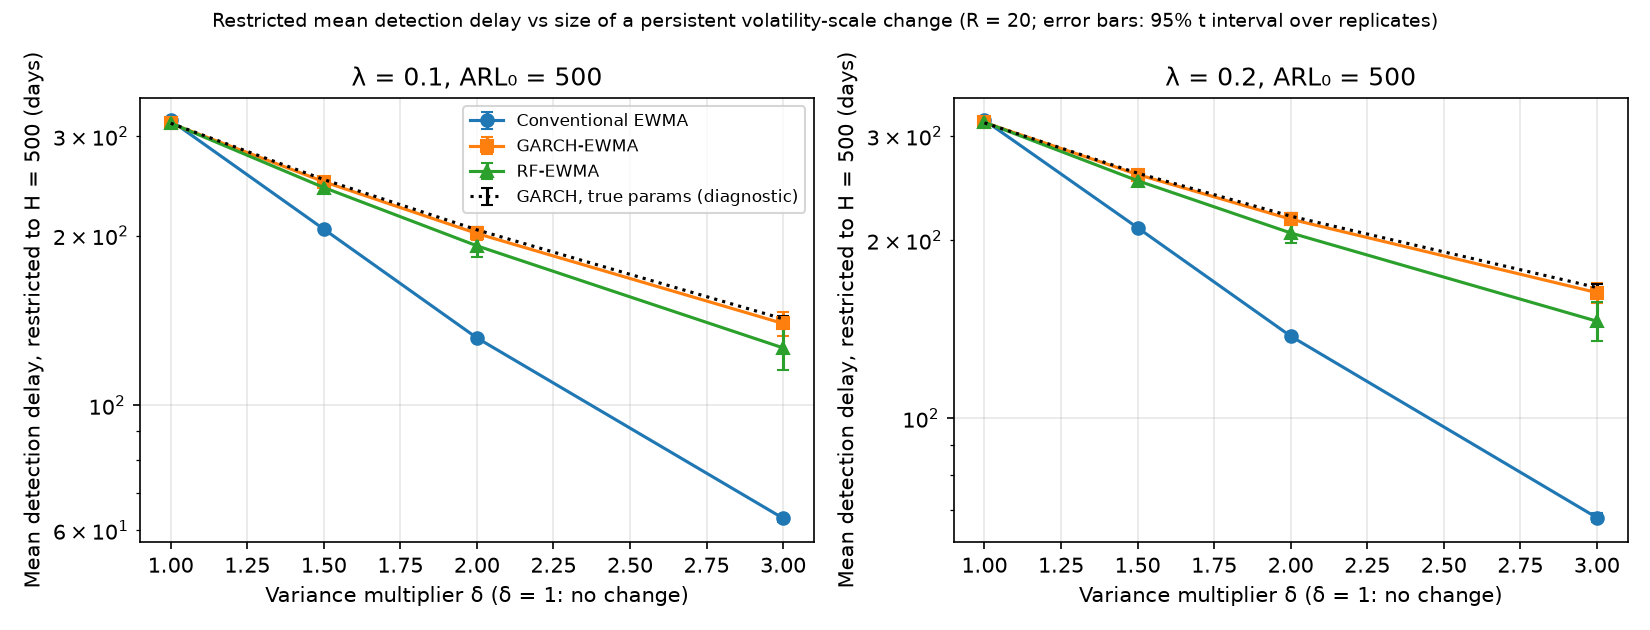
\includegraphics[width=\textwidth]{figures/fig_delay.png}
\caption{Restricted mean detection delay $\RMD$ against the variance multiplier $\delta$ for
$\lambda=0.1$ and $0.2$ (log scale; error bars: 95\% $t$ intervals over $R=20$ systems).}
\label{fig:delay}
\end{figure}

\begin{figure}[htbp]
\centering
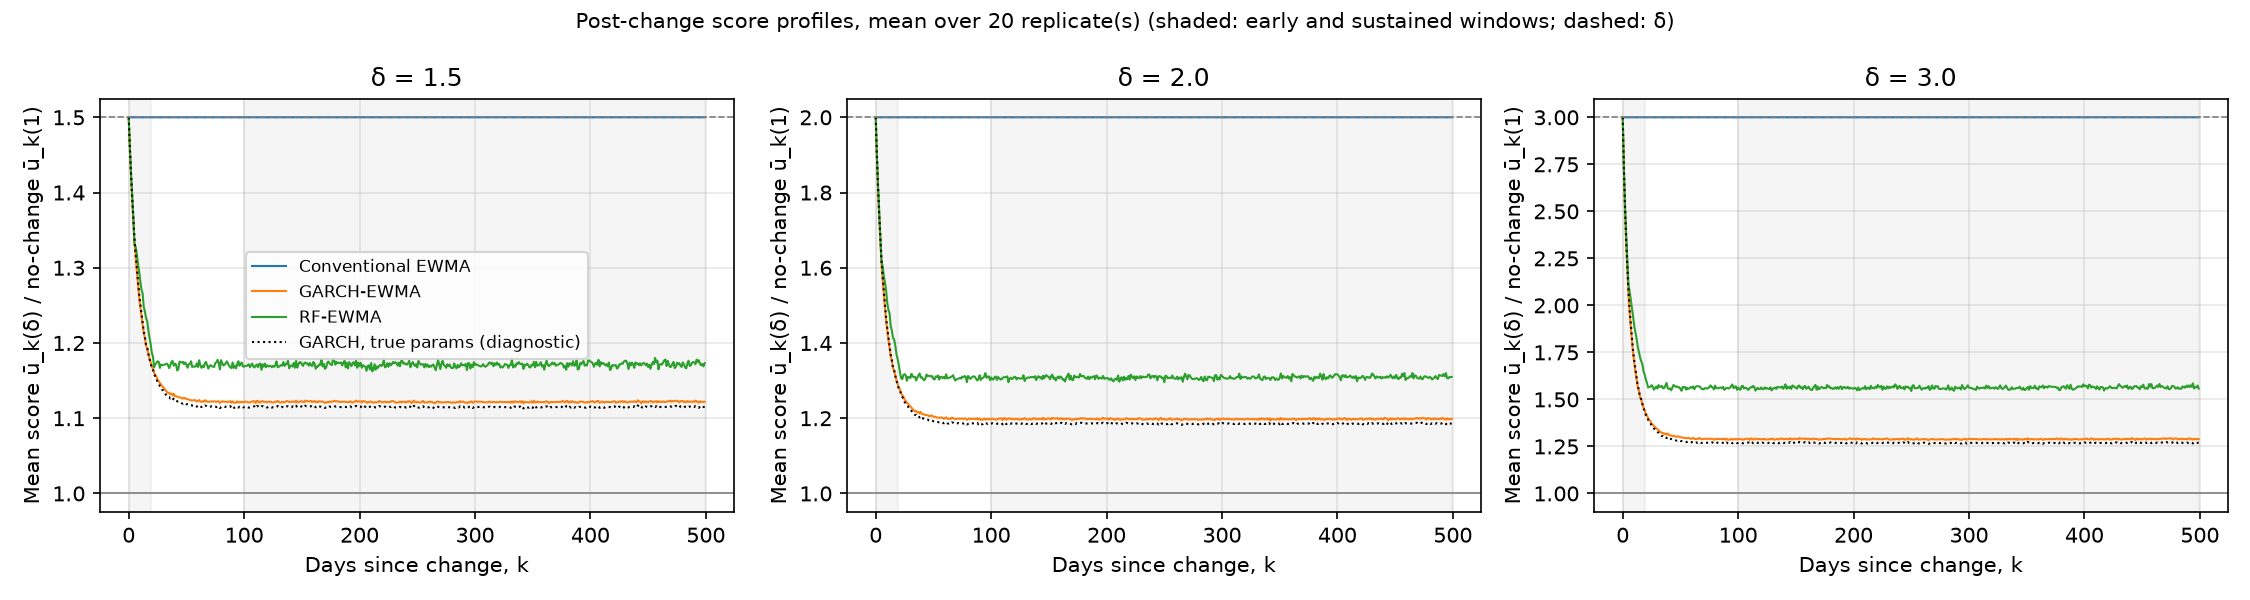
\includegraphics[width=\textwidth]{figures/fig_profile.png}
\caption{Mean post-change monitoring score relative to its no-change value, by days since the change;
shaded: early and sustained windows used for the masking ratio $M$; dashed: $\delta$.}
\label{fig:profile}
\end{figure}

\subsection{Performance comparison}\label{sec:comparison}
% budget: 1 page; the student's Discussion paragraphs close this subsection (within the Section 4 allocation)
\todo{Stage 2: comparison prose. Then the student-written Discussion (outline: the separate writing-outlines document, Section C).}

\begin{table}[htbp]
\centering
\caption{The twelve pre-specified primary paired contrasts ($\lambda=0.1$), with their $\delta=1$ counterparts.
Replicate mean over $R=20$ systems with an unadjusted 95\% $t_{19}$ interval; $+/-$: systems with a positive or
negative contrast.}
\label{tab:contrasts}
\footnotesize\setlength{\tabcolsep}{4pt}
\begin{tabular}{lrcccc}
\toprule
Contrast & Estimate & 95\% CI & $+/-$ & $p$ & Holm $p^{\ddagger}$ \\
\midrule
\multicolumn{6}{l}{\emph{RF $-$ GARCH, RMD$_{500}$ (days)}} \\
\quad $\delta=1$ (no change; context) & 0.27 & [$-$1.24, 1.79] & 9/11 & -- & -- \\
\quad $\delta=1.5$ & $-$6.05 & [$-$10.47, $-$1.63] & 6/14 & 0.010 & 0.053 \\
\quad $\delta=2$ & $-$9.94 & [$-$17.08, $-$2.80] & 5/15 & 0.009 & 0.053 \\
\quad $\delta=3$ & $-$13.13 & [$-$22.88, $-$3.39] & 6/14 & 0.011 & 0.053 \\
\multicolumn{6}{l}{\emph{RF $-$ GARCH, $X(20)$}} \\
\quad $\delta=1$ (no change) & 0 by construction & -- & -- & -- & -- \\
\quad $\delta=1.5$ & 0.0009 & [$-$0.0021, 0.0039] & 10/10 & 0.54 & 1.00 \\
\quad $\delta=2$ & 0.0013 & [$-$0.0027, 0.0054] & 12/8 & 0.50 & 1.00 \\
\quad $\delta=3$ & $-$0.0005 & [$-$0.0092, 0.0081] & 13/7 & 0.90 & 1.00 \\
\multicolumn{6}{l}{\emph{RF $-$ conventional, RMD$_{500}$ (days)}} \\
\quad $\delta=1$ (no change; context) & $-$3.80 & [$-$6.53, $-$1.07] & 5/15 & -- & -- \\
\quad $\delta=1.5$ & 37.54 & [32.96, 42.11] & 20/0 & $5.0\times10^{-13}$ & $6.0\times10^{-12}$ \\
\quad $\delta=2$ & 60.40 & [52.96, 67.84] & 20/0 & $6.0\times10^{-13}$ & $6.6\times10^{-12}$ \\
\quad $\delta=3$ & 63.63 & [53.01, 74.25] & 20/0 & $1.2\times10^{-10}$ & $9.9\times10^{-10}$ \\
\multicolumn{6}{l}{\emph{RF $-$ conventional, $X(20)$}} \\
\quad $\delta=1$ (no change) & 0 by construction & -- & -- & -- & -- \\
\quad $\delta=1.5$ & $-$0.0081 & [$-$0.0110, $-$0.0052] & 1/18 & $1.3\times10^{-5}$ & $9.2\times10^{-5}$ \\
\quad $\delta=2$ & $-$0.0251 & [$-$0.0290, $-$0.0212] & 0/20 & $3.8\times10^{-11}$ & $3.4\times10^{-10}$ \\
\quad $\delta=3$ & $-$0.0608 & [$-$0.0693, $-$0.0524] & 0/20 & $5.3\times10^{-12}$ & $5.3\times10^{-11}$ \\
\bottomrule
\end{tabular}

\par\smallskip\footnotesize\raggedright
$p$: two-sided one-sample $t_{19}$ test of a zero mean contrast. $^{\ddagger}$Supplementary and post hoc: Holm
step-down adjustment over the twelve primary contrasts \citep{holm_1979}, decided after the primary results were
seen; the unadjusted estimates and intervals are the primary results.
\end{table}

\begin{figure}[htbp]
\centering
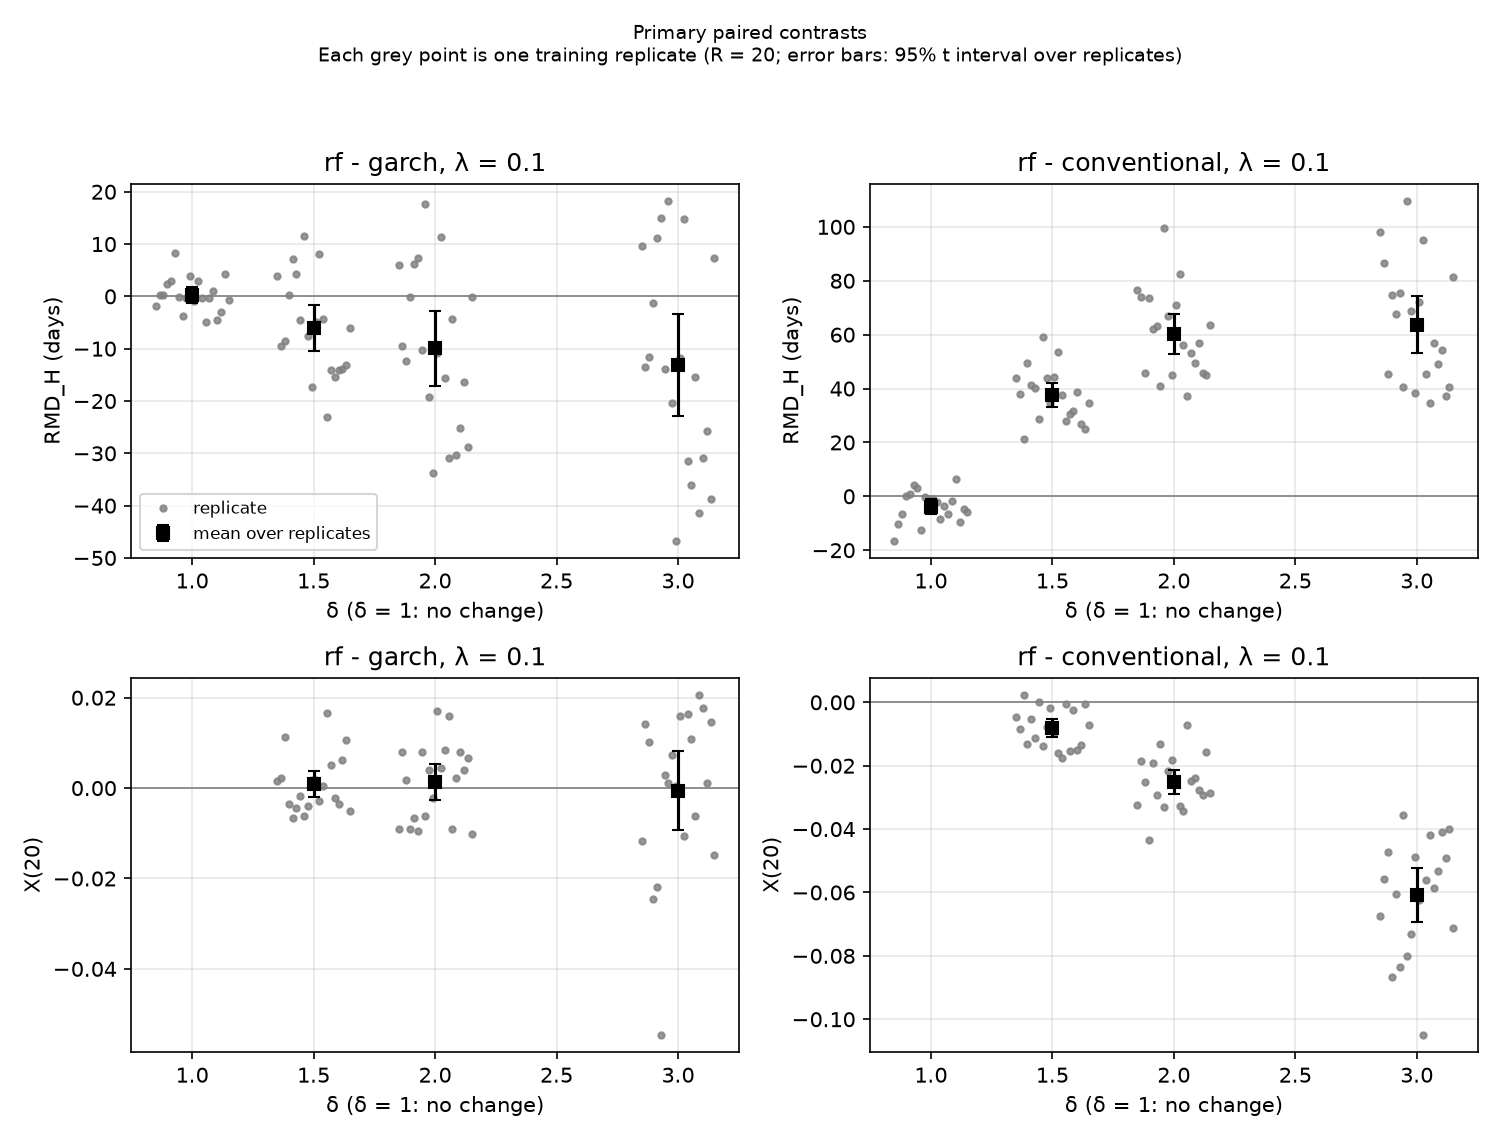
\includegraphics[width=0.85\textwidth]{figures/fig_replicates.png}
\caption{Primary paired contrasts by fitted system: each grey point is one of the $R=20$ systems; squares and
bars: mean and 95\% $t$ interval over systems.}
\label{fig:replicates}
\end{figure}

% ---------------------------------------------------------------- 5 Illustrative example (+/- 2 pages)
\section{Illustrative example: SPY daily returns}\label{sec:spy}
\todo{Stage 2: application prose. Descriptive only.}

\begin{table}[htbp]
\centering
\caption{SPY application: training fits (A) and simulation-calibrated control limits with independent validation (B).
The calibration target is the restricted mean run length $\E[\min(T,5000)]=500$ under the fitted model, not $\E[T]$.}
\label{tab:spyfit}
\small
\textit{(A) Training fits, 1993--2006}\par\smallskip
\begin{tabular}{ll}
\toprule
Quantity & Value \\
\midrule
Training sample (returns) & 1993-02-01 to 2006-12-29 ($n=3507$) \\
Monitoring sample (returns) & 2007-01-03 to 2026-09-30 ($n=4967$) \\
Training variance $s^2$ (\%$^2$) & 1.144 \\
Variance-targeted GARCH(1,1)-$t$ & $\omega=0.0051$, $\alpha=0.0593$, $\beta=0.9363$, $\nu=7.63$ \\
Persistence $\alpha+\beta$ & 0.9955 \\
Fourth-moment coefficient & 1.0039 ($\geq 1$: $E r_t^4=\infty$) \\
RF cell selected (min.\ leaf, max.\ features) & 200, 3 (development QLIKE 0.1872) \\
\bottomrule
\end{tabular}


\medskip
\textit{(B) Control limits and validation}\par\smallskip
\begin{tabular}{cllrlc}
\toprule
$\lambda$ & Chart & $h^*$ & Calibration & Validation [95\% CI] & Eq.~\eqref{eq:val} \\
\midrule
0.1 & Conventional & 1.957 & 500.1 & 483.5 [459.5, 507.5] & pass \\
 & GARCH & 2.598 & 500.1 & 489.2 [468.6, 509.8] & pass \\
 & RF & 2.470 & 500.1 & 477.4 [456.5, 498.3] & pass \\
0.2 & Conventional & 2.870 & 500.6 & 476.4 [452.8, 499.9] & pass \\
 & GARCH & 4.060 & 500.8 & 506.5 [485.4, 527.6] & pass \\
 & RF & 3.901 & 500.2 & 487.7 [466.2, 509.2] & pass \\
\bottomrule
\end{tabular}

\par\smallskip\footnotesize\raggedright
Calibration and validation: restricted mean run length on 2,000 simulated paths each; validation intervals are
conditional on $h^*$.
\end{table}

\begin{figure}[htbp]
\centering
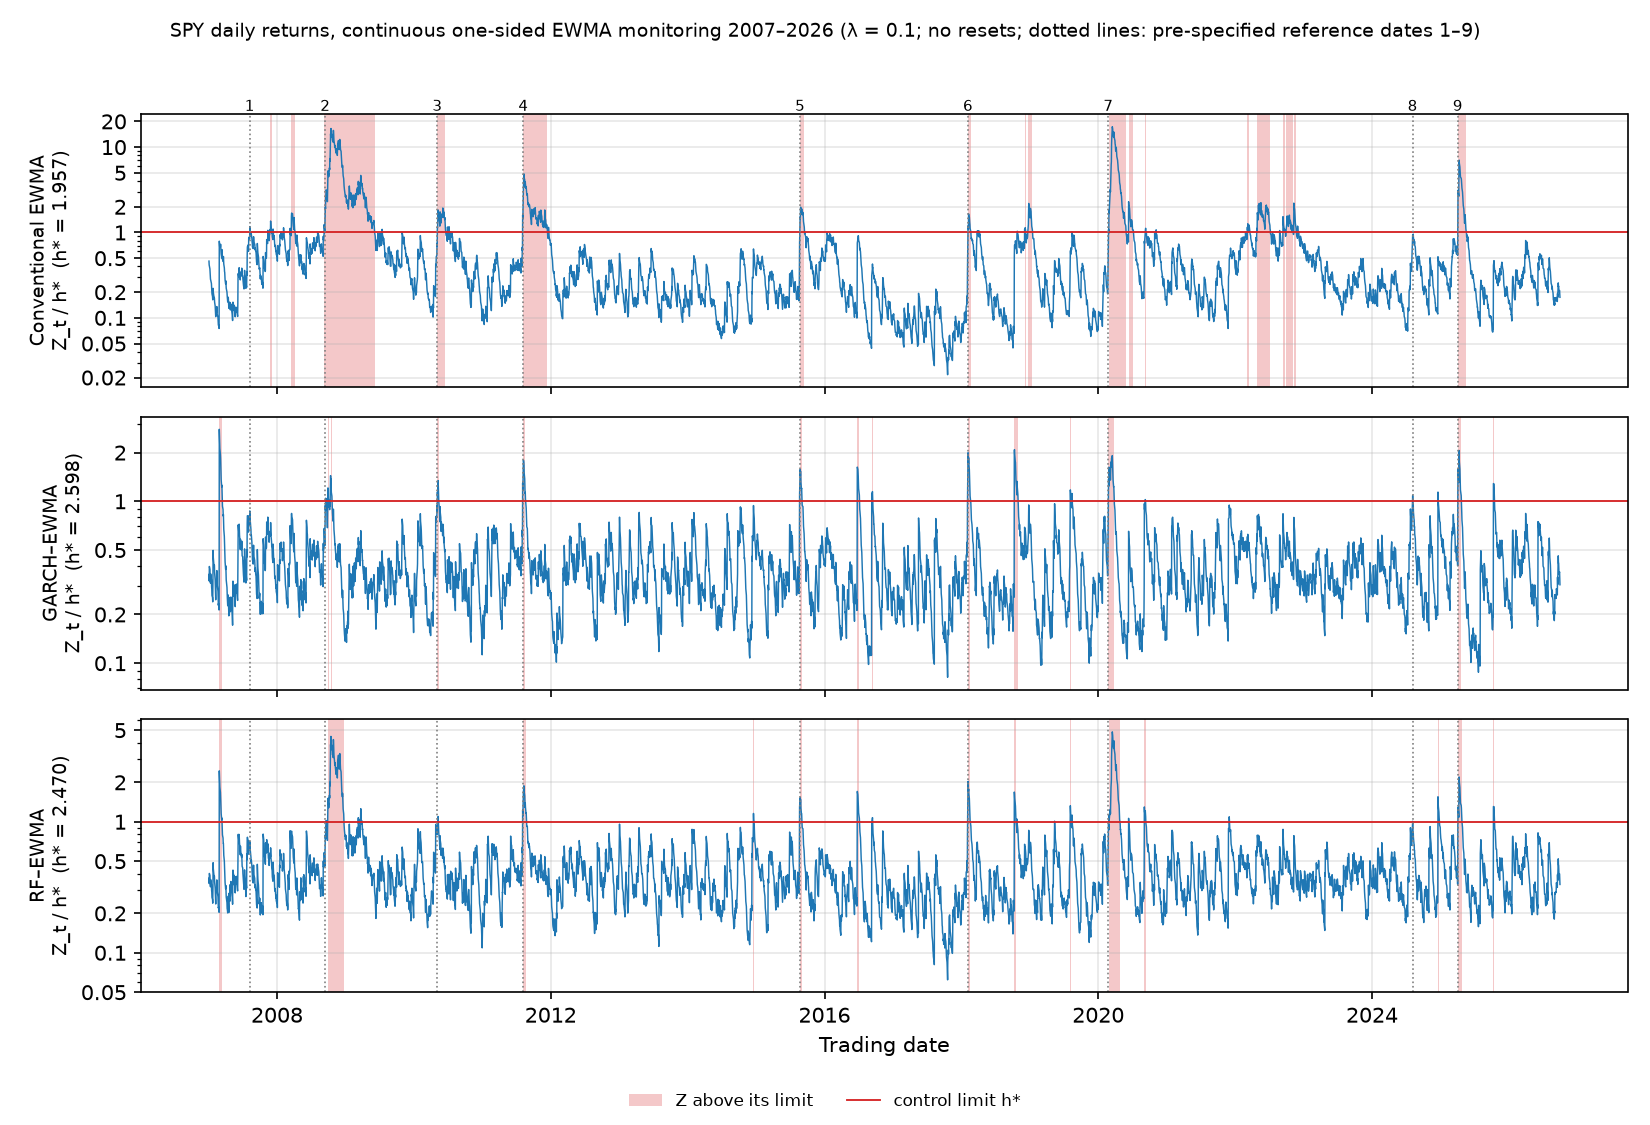
\includegraphics[width=\textwidth]{figures/fig_spy_charts.png}
\caption{SPY 2007--2026: continuous one-sided EWMA statistics relative to their control limits for the three
charts ($\lambda=0.1$; log scale; shaded: days above the limit; dotted: pre-specified reference dates 1--9 of
Table~\ref{tab:spymon}).}
\label{fig:spycharts}
\end{figure}

\begin{table}[htbp]
\centering
\caption{SPY continuous monitoring, 2007-01-03 to 2026-09-30: exceedances and forecast diagnostics (A), and chart
state on the pre-specified reference dates (B). Descriptive only: alarms are not verified changes, and alarm counts
do not rank the methods.}
\label{tab:spymon}
\footnotesize\setlength{\tabcolsep}{4pt}
\textit{(A) Exceedance days, episodes and forecast diagnostics ($\lambda=0.1$ unless stated)}\par\smallskip
\begin{tabular}{lrrrrrrr}
\toprule
Chart & Days above $h^*$ & Episodes & Longest & $\lambda=0.2$: days/episodes & QLIKE & ACF$_1(u)$ & max $d_t$ \\
\midrule
Conventional & 638 (12.8\%) & 44 & 183 & 391 / 58 & 1.462 & 0.273 & 1.14 \\
GARCH & 143 (2.9\%) & 20 & 24 & 77 / 19 & 0.915 & 0.056 & 27.40 \\
RF & 216 (4.3\%) & 27 & 61 & 135 / 23 & 0.986 & 0.115 & 3.37 \\
\bottomrule
\end{tabular}


\medskip
\textit{(B) $Z_t/h^*$ on the date (days to the first exceedance within 63 trading days; --: none)}\par\smallskip
\begin{tabular}{rl>{\raggedright\arraybackslash}p{5.2cm}ccc}
\toprule
\# & Date & Event & Conventional & GARCH & RF \\
\midrule
1 & 2007-08-09 & BNP Paribas suspends three ABS funds & 1.17 (0) & 0.87 (--) & 0.70 (--) \\
2 & 2008-09-15 & Lehman Brothers Chapter 11 filing & 1.97 (0) & 0.94 (2) & 0.79 (4) \\
3 & 2010-05-06 & Flash Crash & 1.14 (0) & 1.14 (0) & 0.94 (2) \\
4 & 2011-08-08 & first session after the S\&P US downgrade & 3.34 (0) & 1.80 (0) & 1.69 (0) \\
5 & 2015-08-24 & China-led global sell-off & 1.52 (0) & 1.57 (0) & 1.53 (0) \\
6 & 2018-02-05 & volatility shock (record VIX jump) & 1.15 (0) & 2.00 (0) & 2.03 (0) \\
7 & 2020-02-24 & COVID-19 sell-off as cases spread outside China & 0.72 (1) & 1.18 (0) & 0.86 (3) \\
8 & 2024-08-05 & yen carry-trade unwind sell-off & 0.94 (--) & 1.09 (0) & 1.01 (0) \\
9 & 2025-04-03 & sell-off after the 2 April tariff announcement & 1.64 (0) & 1.17 (0) & 0.93 (1) \\
\bottomrule
\end{tabular}

\par\smallskip\footnotesize\raggedright
QLIKE against the squared-return proxy $r_t^2$; $d_t$ in \%$^2$. Reference dates were fixed before any SPY
monitoring output existed.
\end{table}

\begin{figure}[htbp]
\centering
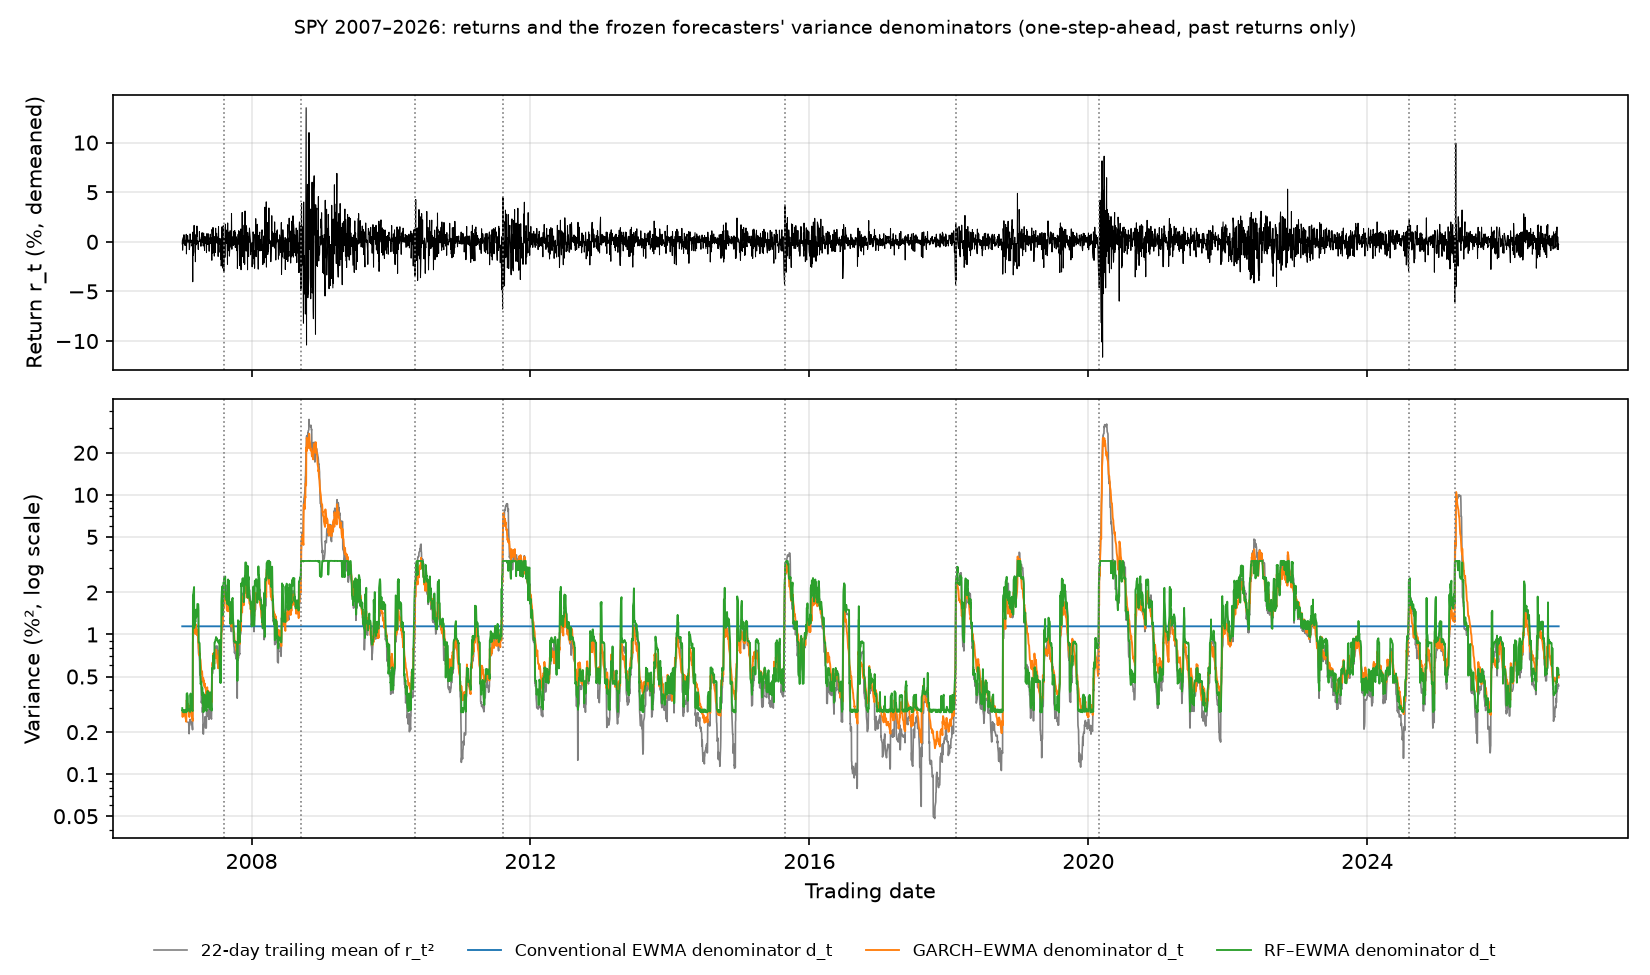
\includegraphics[width=\textwidth]{figures/fig_spy_variance.png}
\caption{SPY 2007--2026: demeaned daily returns (top) and the frozen forecasters' one-step-ahead variance
denominators with a 22-day trailing mean of $r_t^2$ (bottom, log scale).}
\label{fig:spyvariance}
\end{figure}

% ---------------------------------------------------------------- 6 Conclusion (+/- 0.5 page)
\section{Conclusion and recommendations}\label{sec:conclusion}
\todo{Student-written conclusion and recommendations (outline: the separate writing-outlines document, Section D).}

% ---------------------------------------------------------------- Code availability
\section*{Code availability}
The source code used to produce the results in this paper is publicly available at
\url{https://github.com/stephenjamespienaar/stc720-rf-ewma}.

% ---------------------------------------------------------------- References
\nocite{*}  % scaffold only: lists every verified entry; remove once the text cites its sources
\bibliographystyle{apalike}
\bibliography{refs}

\end{document}
